\documentclass[crop, tikz]{standalone}
\usepackage[siunitx, nooldvoltagedirection, american, cute inductors]{circuitikz}
\begin{document}
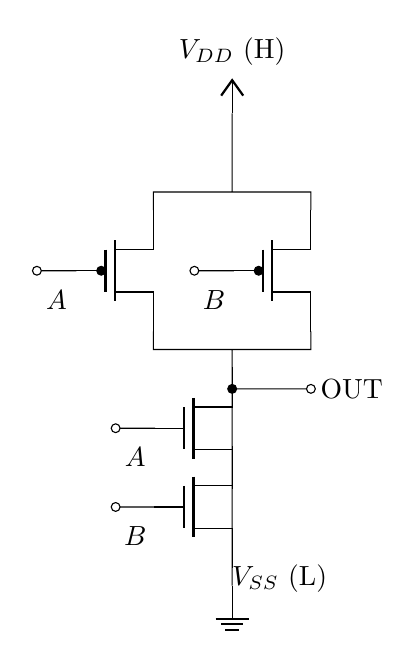
\begin{tikzpicture}
    \draw
    (7,12) node[vcc] {$V_{DD}$ (H)} -- (7,11)
    (6,10) node[pmos] (pa) {}
    (8,10) node[pmos] (pb) {}
    (pa.source) |- (7,11) -| (pb.source)
    (pa.drain) |- (7,9) -| (pb.drain)
    (7,8.5) to[short, *-o] ++ (1,0) node[anchor=west] {OUT}
    (7,9) 
    -- ++ (0,-1) node[nmos] (na) {}
    -- ++ (0,-1) node[nmos] (nb) {}
    -- ++ (0,-1) node[ground] {$V_{SS}$ (L)}
    (pa.gate) to[short, -o, l=$A$] ++ (-0.5,0) node {}
    (pb.gate) to[short, -o, l=$B$] ++ (-0.5,0) node {}
    (na.gate) to[short, -o, l=$A$] ++ (-0.5,0) node {}
    (nb.gate) to[short, -o, l=$B$] ++ (-0.5,0) node {}
    ;
\end{tikzpicture}
\end{document} 